\documentclass[10pt,a4paper]{article}
\usepackage[utf8]{inputenc}
\usepackage[english]{babel}
\usepackage{amsmath}
\usepackage{amsfonts}
\usepackage{amssymb}
\usepackage{listings}
\usepackage{graphicx}
\usepackage{caption}
\author{}
\title{Lazy waiting: an optimized data-flow compiler for Casanova}
\date{}

\lstset
{
	breakatwhitespace = true,
	breaklines = true
	showstringspaces = false,
	basicstyle = \footnotesize\ttfamily ,
	frame = single
}

\begin{document}
\maketitle

\section{Introduction}
\label{sec:introduction}
%%%%%%%%%%%%%%%%%%%%%%%%%%%%%%%%%%%%%%%%%%%%%%%%%%%%%%%%%%
% intro.tex
%%%%%%%%%%%%%%%%%%%%%%%%%%%%%%%%%%%%%%%%%%%%%%%%%%%%%%%%%%

%%%%%%%%%%%%%%%%%%%%%%%%%%%%%%%%
%edit
%%%%%%%%%%%%%%%%%%%%%%%%%%%%%%%%
Computer games promise to be the next frontier in entertainment, with game sales being comparable to movie and music sales in 2010 \cite{ESA}. 

This unprecedented market prospects and potential for computer-game diffusion among end-users has created substantial interest in research on principled design techniques and on cost-effective development technologies for game architectures. Our present endeavour makes a step along these directions. 

Making games is an extremely complex business. Games are large pieces of software with many heterogeneous requirements, the two crucial being high quality and high performance \cite{GAME_OPT}. 


%%%%%%%%%%%%%%%%%%%%%%%%%%%%%%%%
%edit
%%%%%%%%%%%%%%%%%%%%%%%%%%%%%%%%
High-quality in games is comprised by two main factors: visual quality and simulation quality. Visual quality in games has made huge leaps forward, and many researchers continuously push the boundaries of real-time rendering towards photorealism. Simulation quality, on the other hand, is often lacking in modern games; game entities often react to the player with little intelligence, input controllers are used in simplistic ways and the logic of game levels is more often than not completely linear. Building a high-quality simulation is very complex in terms of development effort and also results in computationally expensive code. To make matters worse, gameplay and many other aspects of the game are modified (and often even rebuilt from scratch) many times during the course of development. For this reason game architectures require a lot of flexibility.

To manage all this complexity, game developers use a variety of strategies. Object-oriented architectures, components, reactive progamming, etc have all been used with some degree of success for this purpose \cite{COMPONENTS1,GAMEOBJECTS,FRP}. 

In this paper we will present the Casanova language, a language for making games. Casanova offers a mixed declarative/procedural style of programming which has been designed in order to facilitate game development. The basic idea of the language is to require from the developer only and exclusively those aspects of the game code which are specific to the game being developed. The language aims for simplicity and expressive power, and thanks to automated optimizations it is capable of generating code that is much faster than hand-written code and at no effort for the developer. The language offers primitives to cover the development of the game logic, and incorporates the typical processing of a game engine. Also, the language is built around a theoretical model of games with a ``well-formedness'' definition, in order to ensure that game code is always a good model of the simulated virtual world.

In the remainder of the paper we show the Casanova language in action. We begin with a description of the current state of game engines and game programming in Section \ref{sec:background}. In Section \ref{sec:model} we define our model of games. We describe the Casanova language in Section \ref{sec:casanova}.  We show an example of Casanova in action, and also how we have rewritten the game logic of an official XNA sample from Microsoft \cite{XNA_SAMPLES} in Casanova with far less code and higher runtime performance in Section \ref{sec:case_study}. In Section \ref{sec:conclusions} we discuss our results and some future work.


\section{Case study}
\label{sec:problem_statement}
Networking in games presents a series of standard challenges that we now list and discuss. We will use these challenges as the main reference when doing the evaluation of our networking model. The evaluation, which is discussed in Section \ref{sec:evaluation}, will be a mixture of analytical discussion, user studies, and measured benchmarks.

\subsection{Resource usage}
Available bandwidth [] is quite limited. Noisy wireless networks, poor Internet connections, multiple users sharing a domestic connection, etc. mean that the total bandwidth available to an instance of the game is going to be quite limited. Similarly, latency may be significant for some transmissions, especially if a lot of data is being sent.

The game needs to transmit as little data as possible, for example avoiding the transmission of every updated field, rather relying on mechanisms that locally predict the behaviour of remote entities such as interpolation and  extrapolation.

Similarly, a game needs to be able to present a new, updated picture on the screen at a rate (between 30 and 60 times per second) that is fast enough to give a perception of smoothness. This means that computations for the update and drawing of said picture need to be completed before too much time has elapsed. If networking code is excessively expensive computationally, then it will be impossible for the game to run in real-time.

\subsection{Reliability}
Messages do not always arrive at destination. This may be a temporary issue, for example when some messages are simply lost during transmission. Also, the sudden disappearance from the network of an instance of the game is a common phenomenon. This happens because of unexpected, unintentional difficulties such as electrical interruptions, network cable disconnections, etc., but also because of intentional interruptions: a player may lose interest in the game, or need to leave the game to do something else. Even after a player disconnects, the game may need to keep running: either a new player may be added to fill in for the missing one, or the game will go on just for the remaining players. This means that games need to be resilient to loss of a single instance.

\subsection{Expressive power}
A system designed for building multi-player games should, first and foremost, be expressive enough to cover the definition of various games. Moreover, its semantics should be \textit{appropriate}, meaning that the various idioms of networked communication in games should be easy to express without abusing the available primitives. As such, a mechanism for dealing with networking should offer a simplified view of networking primitives. Such primitives need to be:
\begin{itemize}
\item \textit{few}, because we wish to capture the essential nature of the problem
\item \textit{orthogonal}, because we wish the primitives to have no semantic overlap: each primitive cannot be replaced by the others
\item \textit{intuitive}, because learning to use the system should not require deep understanding through a steep learning curve
\end{itemize}


\section{Casanova overview}
\label{sec:casanova}
Casanova 2 is a declarative-imperative programming language oriented to video game development. A Casanova program is a set of \texttt{entity} definitions organized in a tree structure. The root is a unique entity called \texttt{worldEntity}. Each entity is made of: (\textit{i}) a set of \textit{fields}, \textit{(ii)} a set of \textit{rules}, and (\textit{iii}) a \textit{constructor}. 

A field can have a primitive type (supported types are the most common in other programming languages, such as \texttt{int}, \texttt{float}, \texttt{string}, \textit{tuples}, \textit{lists}) or another entity type. A branch in the tree structure occurs when one field is declared having an entity type. The following example shows a field declaration

\begin{lstlisting}
entity E = {
   A : E1
   B : float
   C : int
   ...
}
\end{lstlisting}

Rules are defined on one or more fields with the keyword \texttt{rule}. A rule can modify the value of fields by using the statement \texttt{yield} on the fields it take as arguments. Besides rules are also passed as implicit arguments the following three values: a reference to the \texttt{worldEntity}, a reference to the current entity (\texttt{this}), and a floating point value (\texttt{dt}) which contains the time difference between the current frame and the previous one. Each rule executes its body continuously, i.e. once the execution has reached the end of the rule body it is resumed from the beginning. The following example shows a rule definition:

\begin{lstlisting}
rule P,V = 
   let new_v = V + g * dt
   let new_p = P + V * dt
   yield new_p,new_v
\end{lstlisting}

A constructor is declared using the keyword \texttt{Create} and may take some parameters as arguments. It returns the initialization of the entity fields enclosed by curly brackets\footnote{This because Casanova 2 syntax is based on F\# syntax and entities are treated as F\# records, thus a constructor returns a record initialization.}. The following example shows a constructor definition:

\begin{lstlisting}
Create(x : E1) =
   {
      A = x
      B = 1.0
      C = 0
      ...
   }
\end{lstlisting}

Casanova 2 supports the most common control structures such as \texttt{if-then-else}, \texttt{while-do}, \texttt{for}, and also SQL-like queries such as (\texttt{for x in list - select - where}). Local variables can be declared using the \texttt{let} statement.

\section{Concurrent operators}
\label{sec:idea}
In this section we describe the general approach of networking in Casanova 2.0. We discuss the architecture, the syntactic and semantic elements, and give a rough idea of how they work. We conclude the section with an in-depth example that shows how to build a small game with a lobby with Casanova 2.0.

\subsection{Architecture}
The architecture of Casanova networking is peer-to-peer. This choice is motivated by the fact that by nature none of the players is significantly more important than the others, and clients may disconnect (because of faults or purposefully because of their users) at all times. A peer-to-peer architecture also has the advantage that each instance is only responsible for a subset of entities: usually those that were generated locally in that instance. A peer-to-peer architecture is compared to a more traditional host-clients architecture where one of the player is the \textit{game host}. The game host usually contains the latest version of the game world, and acts as the latest, authoritative version of the game which all clients are eventually forced to show on their local screens. The advantages of peer-to-peer are various. Peer-to-peer allows us to naturally build systems where computational load is distributed across the various clients. For example, AI that drives the game entities may be run only for the local entities, while the remote ones spawned on the other clients are just synchronized across the net. Also, if a client has transmission problems, then he will not necessarily disrupt the game for all players. Only interactions with him will be problematic, but interactions with other, accessible clients are still possible. In a host-clients architecture, on the other hand, the host is responsible for most computations (such as AI), so the host machine needs to be significantly more powerful than that of the other players. Also, if the host leaves the game, then the game will suffer from issues that range from just quitting the game for all other players, to lengthy waits as a client is promoted to become the new host, etc.

\subsection{Ownership of entities}
In Casanova, entities have a concept of ownership. The instance of the game where an entity is constructed is called the \textit{local} of the entity. The instances of the game that received that entity across the net, on the other hand, are called the \textit{remotes} of the entity. This means that each entity can have two sets of rules: one for its local instance, and one for its remote instances. The local rules will usually (but not necessarily) update the internal logic of the entities that are locally owned, and send (some of) the updates to the remotes. The remote rules will usually (but not necessarily) receives the updates from the local and potentially interpolate the values in order to give a perception of smoothness.

\subsection{Connection primitives}
Casanova supports the concept of connection and disconnection. Each entity may specify what transmissions (or even logic) happens when a new instance of the game connects to the current instances. \textit{local connections} will usually send the locally owned entity to the new instance. \textit{remote connections} will usually receive the remotely owned entity from existing instances, and add it to the game world.

\subsection{Transmission primitives}
In order to be able to send and receive data in a convenient manner, Casanova offers three primitives: \texttt{send}, \texttt{receive},  \texttt{send\_reliable}, and \texttt{receive\_many}. The different versions of \textit{send} are used, respectively, for sending data without confirmation or with confirmation. Confirmation is more expensive in terms of used bandwidth, and can be used when a value \textit{needs} to be transmitted correctly in order to ensure the functioning of the game. The different versions of \textit{receive} are used, respectively, to receive a value from a single instance or from all the current other instances of the game. \texttt{receive\_all} is akin to primitives such as \texttt{gather} in the MPI framework.

Send and receive are generic primitives, meaning that they are capable of full serialization of more complex values. This allows a significant simplification with respect to network libraries which only can transmit elementary data types, because it can be used to hide large and complex transmissions of compound data types without any programmer intervention. This can greatly reduce the amount of bugs that derive from misaligned transmissions such as sending a value on one instance but not receiving it on the other instance. 

Finally, we take advantage of type inference. This means that, even though we could write \texttt{send<T>(x)}, the type inference engine automatically determines, from the parameter \texttt{x} itself, the type \texttt{T}. This allows us to write the much simpler \texttt{send(x)} (the same applies to all other networking primitives).

\subsection{Samples}
In this section we discuss some samples in order to see the Casanova networking primitives in action. We will only show the internal logic of the samples, and the synchronization primitives and the communication protocols. We purposefully avoid showing any rendering code or complex game logic, as that is out of the scope of this work.

\subsubsection{A simple chat}
The first example we see is very simple: an unregulated chat where any new instance of the game can directly add a line to the shared chat lines.

The game world, which represents the main data structure that contains the game data and the rules for a whole instance of the game, is made up of only three fields: the name of the local player, the text of the chat so far, and the text that makes up the line that the local player is writing:

\begin{lstlisting}
world Chat = {
  Name              : string
  Text              : string
  Line              : string
  Keyboard          : Keyboard
\end{lstlisting}

We now specify a series of rules. Rules define how one (or more) fields are updated as time progress in the game or certain events take place (for example key presses). The main rule that governs the dynamics of the chat game will update the \texttt{Line} and \texttt{Text} fields; we see this from the rule header:

\begin{lstlisting}
  rule Line -> Line,Text =
\end{lstlisting}

The rule waits until enter is pressed. When this happens, we send the current \texttt{Line} prefixed by the local user \texttt{Name}. We then reset the local value of \texttt{Line} to the empty string, and add that string to the \texttt{Text}:

\begin{lstlisting}
    wait_until(from c in Line
               exists_by c = '\n')
    send_reliable(Line)
    yield "", Text + Line
\end{lstlisting}

Whenever a character is pressed, then we add it to the line we are writing:

\begin{lstlisting}
  rule Keyboard -> Line =
    wait_until (Keyboard.PressedChars <> [])
    yield Line + Keyboard.PressedChars
\end{lstlisting}

There is also a rule that, in parallel to the previous one, waits until a string is received from one of the other clients and appends it to the \texttt{Text}:

\begin{lstlisting}
  rule Text -> Text =
    yield Text + receive()
\end{lstlisting}

Finally, we specify the \texttt{Create} function that initializes the game world. In this case we take as input the local user name, and use it to initialize the \texttt{Name} field. All other fields start as empty strings:

\begin{lstlisting}
  Create(own_name) = 
    {
      Name     = own_name
      Text     = ""
      Line     = ""
      Keyboard = Keyboard.Create()
    }
}
\end{lstlisting}

\subsubsection{A game lobby}
We now discuss a more complex example: a game lobby (or just \textit{lobby)}. A lobby allows a group of players to coordinate, chat, and in general choose game options right before the game starts. The lobby is an especially interesting case study because it features all elements of a networked game, such as connections, transmissions, and even a bit of non-trivial sequential protocols.

We begin with the lobby data structure. The lobby contains one field for the local player and a list of other (remote) players that are connected to the game:

\begin{lstlisting}
world Lobby = {
  Self     : LobbyPlayer
  Others   : List<LobbyPlayer>
\end{lstlisting}

When a new instance of the game connects to the game, then all existing instances run once the rules inside their \texttt{local connect} scope:

\begin{lstlisting}
  local {
    connect{
\end{lstlisting}

In our case, the existing instances will all reliably send their local players, which are all received with \texttt{receive\_many}. Those players will be stored in the \texttt{Others} list, and used to find a free position for the local player. The local player is then re-created with the new position and sent to the other instances:

\begin{lstlisting}
      rule Self, Others -> Self, Others =
        let others = receive_many()
        let max_x = 
          maxby p in others
          select p.StartPosition.X
        let self = { Self 
                     with Position.X = max_x + 5.0f<pixel> }
        yield +send_reliable(self), others
    }
  }
\end{lstlisting}

The other instances of the game simply do the opposite operation upon connection of a new player, inside the \texttt{remote connect} block.

\begin{lstlisting}
  remote {
    connect {
\end{lstlisting}

First the new instance (reliably) sends its own local player. We receive the new player instance which was just computed remotely and store it locally in the \texttt{Others} list:

\begin{lstlisting}
      rule Self,Others -> Others =
        send_reliable(Self)
        let new_player = receive()
        yield Others + new_player
    }
  }
\end{lstlisting}

We wait until each player declares to be ready, and then we change the game world by switching from the lobby to the main arena:

\begin{lstlisting}
  rule Self,Others -> CurrentWorld = 
    wait_until(Self.Ready)
    wait_until(forall p in Others
               select p.Ready)
    yield Arena.Create(Self)
\end{lstlisting}

When the lobby is created, then it takes as input the string that contains the name of the local player and initializes the players list with only that player (put in the origin):

\begin{lstlisting}
  Create(own_name) = {
    Self   = Players.Create(own_name, Vector2.Zero)
    Others = []
  }
}
\end{lstlisting}

The player entity contains the name of the player, a boolean which signals whether or not that player is ready to play or wishes to remain in the lobby a bit more, and the starting position:

\begin{lstlisting}
entity LobbyPlayer = {
  Name            : string
  Ready           : bool
  StartPosition   : Vector2<pixel>
  Keyboard        : Keyboard
\end{lstlisting}

The entity performs a simple local computation: it waits until the user has pressed the \texttt{Enter} key, and then assigns to its own \texttt{Ready} field the \texttt{true} value. The entity also sends the value \texttt{true} to all of its own remote versions in other instances:

\begin{lstlisting}
  local {
    rule Keyboard, Ready = 
      wait_until Keyboard.EnterPressed
      yield+send_reliable true
\end{lstlisting}

As a safeguard, we also force all players to automatically declare that they are ready after \texttt{30} seconds, in order to avoid players who keep others waiting for too long:

\begin{lstlisting}
    rule () -> Ready = 
      wait(30.0f<s>)
      yield+send_reliable true
  }
\end{lstlisting}

The remote version of the entity in other game instances simply waits to receive its own \texttt{Ready} message, which it assigns locally:

\begin{lstlisting}
  remote {
    rule () -> Ready = 
      yield receive()
  }
\end{lstlisting}

Finally, we create a lobby player from a name and an initial position. The player is initialized as not ready:

\begin{lstlisting}
  Create(name, p) = 
    {
      Name          = name
      Ready         = false
      StartPosition = p
    }
}
\end{lstlisting}


\subsubsection{Game arena}
In this section we discuss how a simple game arena can be defined with Casanova and its networking facilities. In the game we simply have a series of ships, one controlled by the player and others controlled by remote players. When a player shoots, he adds a projectile to his list of locally controlled projectiles. Projectiles are synchronized between instances, so that the projectiles created on an instance are \textit{shown} (but have no real effect on the world) on the other game instances. When an instance of the game registers a hit of one of its \textit{local} projectiles, then it locally adds a \textit{hit} which it also synchronizes with the other instances. When an instance of the game receives a hit on its locally owned ship, then, it registers damage on itself.

In short, \textit{local ships check for messages that tell them they have been hit}, while \textit{hits are registered with the owner of the hitting projectile}.

The arena world contains the ship of the local player and those of the remote players:

\begin{lstlisting}
world Arena = {
  Self		: Ship
  Others	: List<Ship>
\end{lstlisting}

When the instance connects to others, it reliably sends its own local ship and receives the ships of the other instances:

\begin{lstlisting}
  local {
    connect {
      rule Self -> Others = 
      	send_reliable(Self)
      	yield receive_many()
    }
  }
\end{lstlisting}

When the instance connects to others, the others receive its ships and add them to the \texttt{Others} list, and send their own local ship:

\begin{lstlisting}
  remote {
    connect {
      rule Self,Others -> Others = 
      	let new_other = receive()
      	send_reliable(Self)
      	yield Others + new_other
    }
  }
\end{lstlisting}

We create the local instance of the game from the \texttt{LobbyPlayer} that we defined in the previous section. We simply use the starting position to initialize the local ship, and start the instances of the other players as an empty list:

\begin{lstlisting}
  Create(self:LobbyPlayer) =
    {
      Self    = Ship.Create(self.StartPosition)
      Others  = []
    }
}
\end{lstlisting}

The ship entity contains many fields. On one hand, it stores the position, velocity, and health:

\begin{lstlisting}
entity Ship = {
  Position    : Vector2<pixel>
  Velocity    : Vector2<pixel/s>
  Health      : float<health>
\end{lstlisting}

The ship also contains the list of projectiles that it has shot so far:

\begin{lstlisting}
  Shots       : List<Projectile>
\end{lstlisting}

Whenever another ship is hit by one of the local projectiles, then it is added to the list of \texttt{Hits}. The hits are synchronized so that other instances of the game can register damage to their local ships when it is hit by remote instances. Notice that we store the hit ships as \texttt{Ref}, because we just store a pointer to them, which Casanova will then skip when updating and drawing the various entities:

\begin{lstlisting}
  Hits        : List<Ref<Ship>>
\end{lstlisting}

The local instance of a ship updates and sends the position and the velocity with \texttt{yield+send}, which at the same time updates the local value of a field and sends it across the network. Some input-specific code determines how the ship turns and changes direction of movement:

\begin{lstlisting}
  local {
    rule Position,Velocity -> Position = 
      yield+send Position + Velocity * dt
    rule ... -> Velocity = 
      ... input-specific code
      yield+send ...
\end{lstlisting}

The ship also registers its updated health by subtracting the number of hits from others to itself:

\begin{lstlisting}
    rule World.Others, Health -> Health = 
      yield+send(
        Health - from o in world.Others
                 from h in o.Hits
                 where h = Self
                 select 1
                 sum)
\end{lstlisting}

Whenever the ship registers a new shot, it sends it across the network and also stores it to the \texttt{Shots} list:

\begin{lstlisting}
    rule Shots, ... -> Shots = 
      ... input-specific code
      let new_shot = ...
      send(new_shot)
      yield new_shot + Shots
\end{lstlisting}

We split the current shots into two lists. On one hand, we keep the shots which have not yet hit any \texttt{Other} ship and we put them into \texttt{shots'}. On the other hand, we find all the hits that were hit by at least one shot and we put the into \texttt{hits'}. We reliably send these new hits across the network, because we need to communicate to other instances that they need to ``damage themselves'', and we must do so reliably because the hitting event is very important. We also locally keep the new hits and the new shots:

\begin{lstlisting}
    rule Hits,Shots -> Hits,Shots = 
      ... partition Shots into shots and hits
      let hits',shots' = ... 
      send_reliable(hits')
      yield hits', shots'
  }
\end{lstlisting}

Remote instances of a ship receive all the values of updated position, velocity, and health:

\begin{lstlisting}
  remote {
    rule () -> Position = yield receive()
    rule () -> Velocity = yield receive()
    rule () -> Health = yield receive()
\end{lstlisting}

Whenever a new shot is received, then it is added to the local list:

\begin{lstlisting}
    rule Shots -> Shots = 
      let new_shot = receive()
      yield new_shot + Shots
\end{lstlisting}

Whenever a new set of shots is received, we wait for a tick (so that they can be processed by reducing the health of the local ship as needed) and then remove them:

\begin{lstlisting}
    rule () -> Hits = 
      yield receive()
      yield []
  }
\end{lstlisting}

Inactive shots are removed from the list of shots. This is done outside either the \texttt{local} or the \texttt{remote} blocks, and as such even remote instances of a ship will remove inactive projectiles:

\begin{lstlisting}
  rule Shots -> Shots = 
    from s in Shots
    where s.Active
    select s
\end{lstlisting}

We create a ship from an initial position and with full health, no shots, and no hits:

\begin{lstlisting}
  Create(p) =
    {
      Position = p
      Velocity = Vector2.Zero
      Health   = 100.0<health>
      Shots    = []
      Hits     = []
    }
}
\end{lstlisting}

The projectile, similarly to the ship, contains a position, a velocity, and an \texttt{Active} flag to determine when the projectile is to be removed:

\begin{lstlisting}
entity Projectile = {
  Position    : Vector2<pixel>
  Velocity    : Vector2<pixel/s>
  Active      : bool
\end{lstlisting}

All projectiles, regardless of whether they are local or remote, update their position according to the usual physical rules:

\begin{lstlisting}
  rule Position,Velocity -> Position = 
    yield Position + Velocity * dt
\end{lstlisting}

The local instance of a projectile sends, every few seconds, the position and the velocity to the remote instances:

\begin{lstlisting}
  local {
    rule Position -> Position =
      wait 5.0<s>
      send(Position)
    rule Velocity -> Velocity =
      wait 10.0<s>
      send(Velocity)
\end{lstlisting}

After twenty seconds the projectile is registered both locally and remotely as inactive:

\begin{lstlisting}
    rule () -> Active =
      wait 20.0<s>
      yield+send_reliable false
  }
\end{lstlisting}

The remote versions receive the sent values:

\begin{lstlisting}
  remote {
    rule () -> Position = 
      yield receive()
    rule () -> Velocity =
      yield receive()
    rule () -> Active =
      yield receive()
  }
\end{lstlisting}

Finally, we create a projectile from its position and velocity, and we set it to \texttt{Active}:

\begin{lstlisting}
  Create(p,v) =
    {
      Position = p
      Velocity = v
      Active   = true
    }
}
\end{lstlisting}


\subsubsection{Disconnection}
Disconnection is not handled with explicit primitives. Rather, disconnection can be handled with a mixture of the networking primitives that we have seen so far and the default primitives that Casanova offers.

We add to the entity that handles disconnection a boolean flag and a time stamp. One flag is for disconnection, the other is for pings:

\begin{lstlisting}
Disconnected : bool
LastPing     : Time
\end{lstlisting}

The local instance of an entity sends a ping every few seconds that signals that the entity is not disconnected. The ping is of type \texttt{Unit}, meaning that it contains no data whatsoever:

\begin{lstlisting}
local {
  rule () -> LastPing =
    wait 5.0<s>
    send()
}
\end{lstlisting}

The remote instance reads the ping messages and resets the last ping time whenever it receives something:

\begin{lstlisting}
remote {
  rule () -> LastPing =
    receive()
    yield Now()
\end{lstlisting}

If no ping has been received within a reasonable time, then we set the \texttt{Disconnected} flag to true:

\begin{lstlisting}
  rule LastPing -> Disconnected =
    wait (Now() - LastPing > 30.0<s>)
    yield true
}
\end{lstlisting}

As a side note, when an instance is communicating with another one from \textit{inside a rule}, within a complex protocol, then in case of disconnection between one of the parties the rule execution will be aborted midway. This is needed in order to prevent protocols stuck midway (after the other party disconnected) and stealing messages from other communications.

\subsubsection{Verbose syntax}
In some cases, the type of the message is ambiguous inside an entity. For example, when transferring multiple boolean flags, the language may be unable to understand when to receive one message or the other.

Consider an entity that contains two boolean fields, \texttt{A} and \texttt{B}:

\begin{lstlisting}
A : bool
B : bool
\end{lstlisting}

The local instance of the entity updates \texttt{A} and \texttt{B} according to some internal logic, such as input, AI, etc.:

\begin{lstlisting}
local {
  ... logic for updating A and B
\end{lstlisting}

Both \texttt{A} and \texttt{B} are sent across the network to the remote instances:

\begin{lstlisting}
  rule A -> A = yield+send(A)
  rule B -> B = yield+send(B)
}
\end{lstlisting}

The remote instances try to receive \texttt{A} and \texttt{B}, but the compiler has no way to determine what the intention of a message was:

\begin{lstlisting}
remote {
  rule () -> A = yield receive()
  rule () -> B = yield receive()
}
\end{lstlisting}

It may seem intuitively reasonable to match sends and receives depending on the rule name, but this can lead to a system which is too restrictive: it may be that the developer really wishes to swap \texttt{A} and \texttt{B} between the local and the remote.

A better solution is to give a compiler error for ambiguous cases, and at the same to offer explicit \texttt{send} and \texttt{receive} primitives with a user-defined \textit{label}. Ambiguous communication operations will be matched depending on the label, and not only on the type:

\begin{lstlisting}
send[ID]<T>(E:T) : Unit
receive[ID]<T>() : T
\end{lstlisting}

The example above would then become:

\begin{lstlisting}
local {
  rule A -> A = yield+send[A]<bool>(A)
  rule B -> B = yield+send[B]<bool>(B)
}

remote {
  rule () -> A = yield receive[A]<bool>()
  rule () -> B = yield receive[B]<bool>()
}
\end{lstlisting}

Notice that we could also use labels which are not related to the names of the fields which are sent, for example to have more descriptive sources in the case where we swap the values of \texttt{A} and \texttt{B} \footnote{Imagine that \texttt{X} and \texttt{Y} are descriptive labels that capture the essence of the communication.}:

\begin{lstlisting}
local {
  rule A -> A = yield+send[X]<bool>(A)
  rule B -> B = yield+send[Y]<bool>(B)
}

remote {
  rule () -> A = yield receive[Y]<bool>()
  rule () -> B = yield receive[X]<bool>()
}
\end{lstlisting}

\paragraph{A more complex motivation}
Sending and receiving with an explicit ID for the operation is an advanced feature that is most often needed in complex scenarios. For this reason it is relatively hard to come up with a convincing, yet simple, example that uses it. It is possible, on the other hand, to describe the abstract class of game rules that may benefit from this kind of computation.

Suppose that we have two fields in an entity. Field \texttt{A} is a boolean, and as such can be transmitted easily across instances with minimal bandwidth usage. Field \texttt{X}, on the other hand, has type \texttt{T}, which we assume to be \textit{too large} to transmit often across the network:

\begin{lstlisting}
A : bool
X : T
\end{lstlisting}

There are a series of similar rules that all compute a new value for \texttt{A}, and use that value to compute a new value for \texttt{X}. Each rule uses a different way to compute both \texttt{A} and \texttt{X}:

\begin{lstlisting}
local {
  rule A,X -> A,X = 
    let A' = a1()
    let X' = f1(A')
    yield +send(A'), X'
  rule A,X -> A,X = 
    let A' = a2()
    let X' = f2(A')
    yield +send(A'), X'
  ...
  rule A,X -> A,X = 
    let A' = aN()
    let X' = fN(A')
    yield +send(A'), X' 
}
\end{lstlisting}

When we receive a value of \texttt{A}, we can compute the correct value of \texttt{X} without having to transmit it: 

\begin{lstlisting}
remote {
  rule X -> A,X = 
    let A' = receive()
    let X' = f1(A')
    yield A', X'
  rule X -> A,X = 
    let A' = receive()
    let X' = f2(A')
    yield A', X'
  ...
  rule X -> A,X = 
    let A' = receive()
    let X' = fN(A')
    yield A', X'
}
\end{lstlisting}

Unfortunately, the system has no way of determining which \texttt{send} is paired with which \texttt{receive}. For this reason we will have to tag each transmission with an appropriate ID to disambiguate:

\begin{lstlisting}
local {
  rule X -> A,X = 
    let A' = a1()
    let X' = f1(A')
    yield +send[ID1](A'), X'
  rule X -> A,X = 
    let A' = a2()
    let X' = f2(A')
    yield +send[ID2](A'), X'
  ...
}

remote {
  rule X -> A,X = 
    let A' = receive[ID1]()
    let X' = f1(A')
    yield A', X'
  rule X -> A,X = 
    let A' = receive[ID2]()
    let X' = f2(A')
    yield A', X'
  ...
}
\end{lstlisting}

Thanks to this disambiguation the system now knows that the various \texttt{send} operations will only feed data in the appropriate \texttt{receive} slots.


\section{Operators optimization}
\label{sec:details}
\begin{itemize}
\item Static analysis technique to detect dependencies.
\item We use these dependencies to generate data structure for scheduling interrupted rules.
	\begin{itemize}
	\item Each entity maintains a list of entities depending on it, and a list of inactive rules.
	\item Maintaining the list according to the dynamics of entities in the game (creation, update, and removal).
	\end{itemize}
\item To what extent a game can benefit from such an optimization? Game state changing too fast. Optimization data structures create overhead which surpass the performance gained by our scheduling.
\item Dynamic analysis technique to detect the update frequency.
\item Rules that update too often will not benefit from our optimization and are not included.
\item The choice of the update threshold depends on the data structure we are using for the optimization.
\item Further optimization: data structures can be stored in the world instead of locally into entities for better cache coherence.
\end{itemize}

A problem that arises from the use of some of these operators is that of \textit{busy waiting}. For instance, the healer behaviour requires that he waits for a guard to ask for healing before leaving the guard post. To describe this behaviour we must continuously check if a wounded guard is nearby. The overhead of this operation is minimum for just one guard, but for a greater amount of guards this can seriously affect the game performance, since it is required that the healer checks if any guard is close enough at every game frame. This observation can be generalized for rules which wait for a condition on values of the game state altered by other rules. Consider the following example in Casanova 2:

\begin{lstlisting}[mathescape]
entity E = {
   A : int
	
   rule A = //rule $r_{1}$
      wait 1.0
      yield A + 1
   rule A = //rule $r_{2}$
      wait A % 2 = 0
      //execute rule body $b_{2}$
   rule A = //rule $r_{3}$
      wait A % 5 = 0
      //execute rule body $b_{3}$
   rule A = //rule $r_{4}$
      wait A % 10 = 0
      //execute rule body $b_{4}$
      
   Create() = {A = 0}		
}
\end{lstlisting}
In the snippet of code shown above, rule $r_{1}$ increments the field A by 1 every second. Rules $r_{2}$, $r_{3}$, and $r_{4}$ wait until A is multiple of respectively 2, 5, and 10 before executing the rest of their bodies. If we assume that running rule bodies $b_{2}$, $b_{3}$, and $b_{4}$ take 0.5 seconds, and we consider a time span of 12 seconds, then $r_{2}$ will be inactive for 10 seconds and run for 2 seconds, $r_{3}$ will be inactive for 11 seconds and run for 1 seconds, and $r_{4}$ will be inactive for 11.5 seconds and active for 0.5 seconds. This comparison is shown in Figure \ref{fig:s4f1}. The time amount in the light grey bars is spent by rules by busy waiting, since in that time interval they keep checking the synchronization condition. We observe that the reactivation of a rule body execution depends only on a change on the fields used in the boolean expression of the \texttt{wait} operator, and this change can only be performed by other active rules (in our example only $r_{1}$, but in a more general case there could be more than one rule acting on the same field). From this consideration we argue that we can make waiting dependent on the game state rather than on the rule state.

\begin{figure}
	\centering
	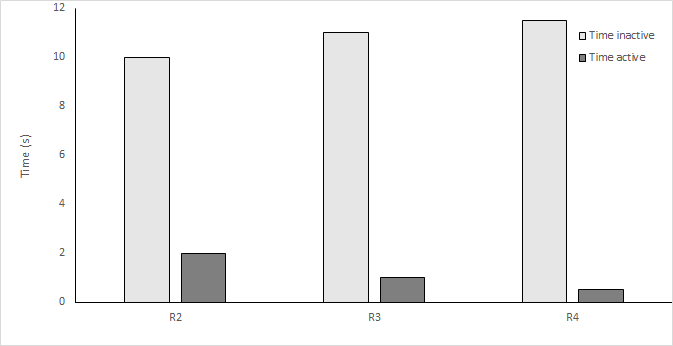
\includegraphics[scale=0.5]{Image/wait_chart}
	\caption{Chart showing the time spent by inactive and active rules}
	\label{fig:s4f1}
\end{figure}

Given that the evaluation of a waiting condition changes only when at least one of the fields affecting it has changed, we keep track of all rules waiting for a change on that field (this can be done statically by examining the expression of a \texttt{wait} operator). When a rule evaluates the condition of a \texttt{wait} operator, if the condition evaluates to \texttt{false}, it is suspended. When another rule changes a field, it resumes any suspended rules with that field. Suspended rules evaluate again the \texttt{wait} conditions. Those which evaluate to \texttt{false} remain suspended, those which evaluate to \texttt{true} become active again and proceed with their execution.

The other operators affected by busy waiting are the concurrency operator and the pre-emption operator (the parallel operator keeps executing its code continuously and it does not wait for any condition itself, although its body can contain other operators that do).

\section{Evaluation}
\label{sec:evaluation}
We now present an RTS game we used as a case study, created with Casanova, and the benchmarks that test the action implementation. In the game players must conquer a star system made up of various planets. Each planet builds fleets which are used to fight the fleets of the other players and to conquer more planets. A planet is conquered when a fleet of a player is near it and no other enemy fleet is defending it.

\subsection{Case study}

Three actions are required in this game: The first action, called \texttt{Fight Action}, defines how a fleet fights enemy fleets in range. The fight action subtracts $0.5 \cdot dt$ \texttt{life} points from the in-range enemy fleet during every frame (action tick).

\begin{lstlisting}[language=Caml]
Fleet = {Position: Rule Vector2;FightAction: FightAction;Owner: Ref Player;Life: Var float32;Fight: FightAction }
\end{lstlisting}

The Fight Action is defined as follows:

\begin{lstlisting}[language=sql]
FightAction = TARGET Fleet; RESTRICTION Owner <> Owner; RADIUS 150.0; TRANSFER CONSTANT Life - 0.5;
\end{lstlisting}

The target is an entity of which the type is \textbf{Fleet}. The condition to execute the action is that the fleet must be an enemy (i.e., not the player). The \texttt{attack range} is 150 units of distance. 0.5 \texttt{life} points are subtracted for every attack.

The second action is called \texttt{BuildAction}. It allows a planet to create a ship. In order to build a ship, a planet must gather 10 mineral units. Each planet has a field called \texttt{GatherSpeed} which determines how fast it gathers minerals. Every tick the planet's mineral stash is increased by this amount. This action is a threshold action where the threshold value is the minerals of the planet. As soon as the threshold value is reached, we set the field \texttt{NewFleet} to TRUE (it is used by the engine to create a new fleet), and \texttt{Minerals} to 0 to reset the counter. The planet and its actions are:

\begin{lstlisting}[language=Caml]
Planet = {Position: Vector2;Owner: Rule Ref Player;NewFleet: Rule bool;BuildAction:BuildAction;EnemyOrbitingFleetsAction : EnemyOrbitingFleetsAction;GatherSpeed: float32;Minerals: Var float32 }
\end{lstlisting}

\begin{lstlisting}[language=sql]
BuildAction =
TARGET Self; TRANSFER CONSTANT Minerals + GatherSpeed; THRESHOLD Minerals 10.0; OUTPUT NewFleet := true; OUTPUT Minerals := 0.0
\end{lstlisting}

A Casanova rule is appointed to read the value of NewFleet and, when it is true, to spawn a new fleet.

The third action is required to check if a planet can be conquered by a fleet. A fleet can conquer a planet if there is no enemy fleet near it and if it is sufficiently close. Thus the action definition is the following:

\begin{lstlisting}[language=sql]
EnemyOrbitingFleetsAction =
TARGET Fleet; RESTRICTION Owner Not Eq Owner; RADIUS 25.0; INSERT Owner -> EnemyOrbitingFleets
\end{lstlisting}

The action will add an enemy fleet close enough to change the owner of the planet.

%Even the concept of drawing lasers can be implemented using the INSERT clause simply adding it to \texttt{FightAction} which inserts in a list all the targeted ships positions. In this way we can draw a laser from the source position to the target position. We omit this aspect for brevity.

\subsection{Evaluation}

We evaluated the performance of our approach with the case study, and two extra examples: an asteroid shooter, and an expanded version of the case study with more complex rules. All were implemented in Casanova. Table \ref{tab:code_length} shows a code length comparison between the REA implementation and standard Casanova rules for all three.

We note that in games with basic dynamics the code saving is low, due to the fact that there are few repeated patterns. The advantage of using REA becomes evident in a game with actions involving many types of targets, such as the expanded case study. Furthermore, we managed to drastically increase the performance of the game logic: as Figure \ref{fps_chart} shows, using REA (labeled ``with actions'') results in a speedup factor of 6 to 25, due to automated optimizations in the query evaluation. We also note that our implementation is flexible and general since it is possible to use actions to express a behaviour, such as a projectile collision, which is outside the domain of RTS games and traditional resource-based systems.

\begin{table}
\centering
\caption{CS (case study), Asteroid Shooter and Expanded CS code length}
\label{tab:code_length}
\begin{tabular}
{|l|c|c|c|c|c|c|}
\hline
& Game Entities & Rules & Actions & Total\\
\hline
\textit{CS with REA} & 41 & 71 & 19 & 131\\
\hline
\textit{CS without REA} & 40 & 90 & 0 & 130\\
\hline
\textit{Asteroid shooter with REA} & 33 & 33 & 6 & 72\\
\hline
\textit{Asteroid Shooter without REA} & 34 & 44 & 0 & 78\\
\hline
\textit{Extended CS with REA} & 135 & 138 & 40 & 313\\
\hline
\textit{Extended CS without REA} & 135 & 328 & 0 & 463\\
\hline
\end{tabular}
\end{table}
\begin{figure}
\centering
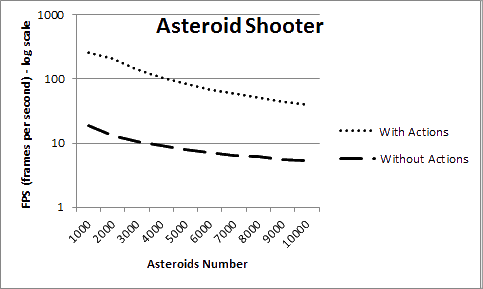
\includegraphics[scale=0.7]{Shooter.png}
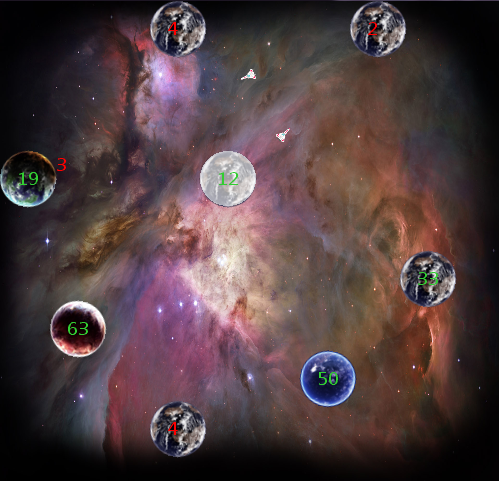
\includegraphics[scale=0.7]{RTS.png}
\caption{Frame rate as a function of numbers of entities.}
\label{fps_chart}
\end{figure} 

\section{Related works}
\label{sec:related_works}
\input{related_works}

\section{Future works}
\label{sec:future_works}
\begin{itemize}
\item Wait scheduling based on time: evaluate only the next-to-happen wait in our time frame.
\item Improve the dynamic optimization.
\item Hierarchical dependencies in the static optimization.
\item Statistical analysis on dependencies.
\end{itemize}

\section{Conlcusions}
\label{sec:conclusions}
%% Changed by PS, April 4, 2014.

\section{Future work}
\label{sec:future_work}
The Casanova 2 language is capable of implementing usable and quite complex games. The language, while usable, is currently still in development as it misses a few features. In particular, support for multiplayer games is at this moment lacking. We believe that the existing mechanisms for handling time offered by Casanova 2 could be augmented with relatively little effort in order to greatly simplify the hard task of building multiplayer games. This is part of future work, that we are currently engaging in. We are also doing usability studies using students from various disciplines and backgrounds.

The high level view of the game that the Casanova 2 compiler provides can be exploited in order to improve the programmer experience. This means that we could use tools for code analysis (such as abstract interpretation \cite{nielson1999principles} or type system extensions) in order to better understand the game being built, and to help with correctness analysis, performance analysis, or even optimization.


%\subsection{User study}
%We wish to perform an in-depth user study for Casanova 2 to improve usability in the development process. We have already performed a partial (and quite promising) small user study which we will extend and complete.


%We have performed the following test: we gathered a group of students of game programming and a group of students of game design. We gave them a series of Casanova 2 samples, printed on paper. Each student had to guess the functionality of each sample, and sketch a screen-shot. Furthermore, each student also provided some additional feedback on the language.

%The samples were: (\textit{i}) a string of text moved around the screen with the keyboard, (\textit{ii}) a string of text that moves along a predefined path automatically, and (\textit{iii}) an asteroid shooter.

%Eleven (over a total of thirteen) students understood the samples completely, both drawing the screen-shots and explaining the dynamics of the game correctly. Two students were lost on the syntactic differences between Casanova 2 and the more familiar C-like syntax. The direct feedback was mostly centred around a series of common observations, which are reported in Table \ref{students_feedback}. For each observation, the table reports how many times we encountered it.

%\begin{table}[!t]
%% increase table row spacing, adjust to taste
%\renewcommand{\arraystretch}{1.3}
% if using array.sty, it might be a good idea to tweak the value of
% \extrarowheight as needed to properly center the text within the cells

%\caption{Feedback from students}
%\label{students_feedback}
%\centering

%% Some packages, such as MDW tools, offer better commands for making tables
%% than the plain LaTeX2e tabular which is used here.
%\begin{tabular}{|c||c|}
%\hline
%Syntax is unfamiliar at first & 3\\
%\hline
%Syntax is clear & 8\\
%\hline
%Indentation instead of parentheses is a downside & 2\\
%\hline
%List processing with queries is very effective & 1\\
%\hline
%Rules are a good abstraction for games & 2\\
%\hline
%\end{tabular}
%\end{table}

%We also built a significantly bigger sample, which we asked only three students to study. The sample is a checkpoint-based RTS (see Figure \ref{RTS game} for a screenshot). All students correctly identified the game mechanics, and provided some additional feedback. Most of this feedback overlaps with that obtained for the samples, but some new observations emerge. Arguably, some patterns become visible only with larger samples:
%\begin{itemize}
%\item \texttt{wait} and \texttt{when} are very powerful
%\item Multiple rules on the same field are very powerful
%\item Multiple rules on the same field may lead to behaviours that are complex to understand
%\end{itemize}


\section{Conclusions}
\label{sec:conclusions}

Casanova 2, a language specifically designed for building computer games, may offer a solution for the high development costs of games. The goal of Casanova 2 is to reduce the effort and complexities associated with building games. Casanova 2 manages the game world through entities and rules, and offers constructs (wait and yield) to deal with the run-time dynamics. As shown by the benchmarks in Section \ref{sec:evaluation}, we believe that we have taken a significant step towards reaching these goals. In fact, we achieved at the same time very good performance and simplicity, thereby empowering developers with limited resources. 


\end{document}